\begin{center}
    {\LARGE \textbf{2011有机化学}} \\[2ex]
    {\large 时量180分钟 \quad 满分150分}
\end{center}

\vspace{0.5cm}
\noindent\textbf{注意事项:}
\begin{enumerate}[label=\arabic*., parsep=0pt, itemsep=0pt]
    \item 答题前,考生先将自己的姓名、学号、考场号、座位号填写在答题卡上,将条形码准确粘贴在考生信息条形码粘贴区。
    \item 考试结束后,将本试卷与答题纸一并收回。
    \item 回答各个问题时,将答案写在答题纸上,写在本试卷上无效。
\end{enumerate}

\vspace{0.5cm}
\noindent\textbf{一、完成反应(50 pts.)}

\begin{enumerate}[label=\arabic*., itemsep=3ex]
    \item 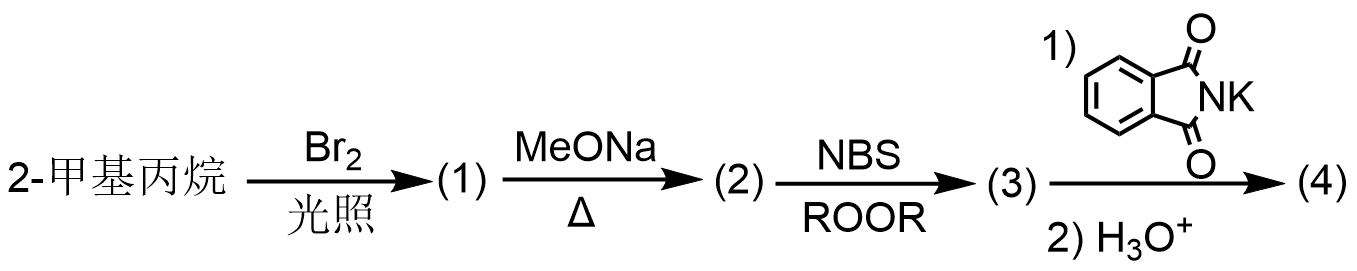
\includegraphics[scale=0.38, valign=c]{./Figure/2011/2011_1_1.png} 
    \item 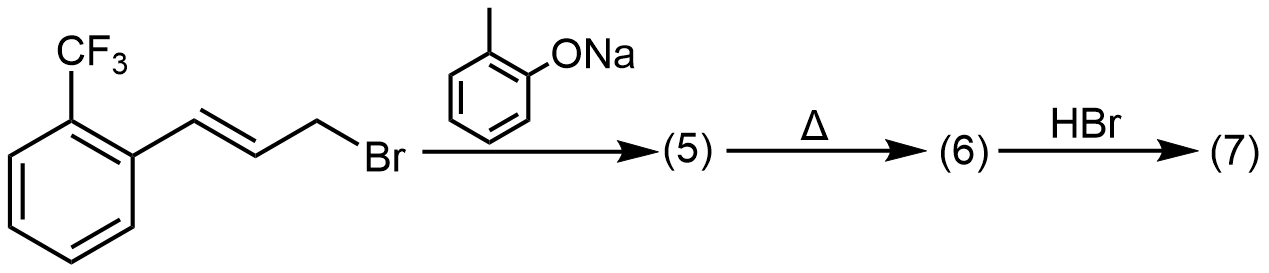
\includegraphics[scale=0.38, valign=c]{./Figure/2011/2011_1_2.png}
    \item 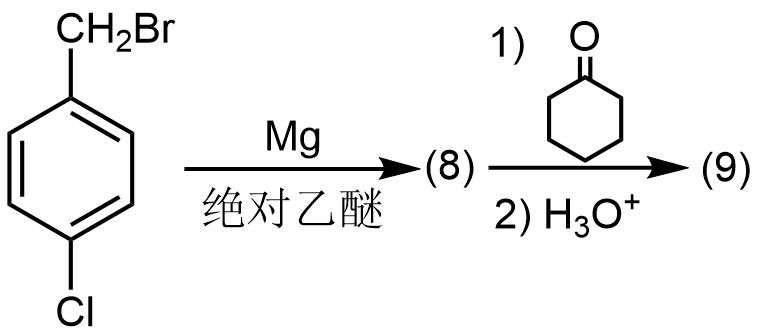
\includegraphics[scale=0.38, valign=c]{./Figure/2011/2011_1_3.png}
    \item 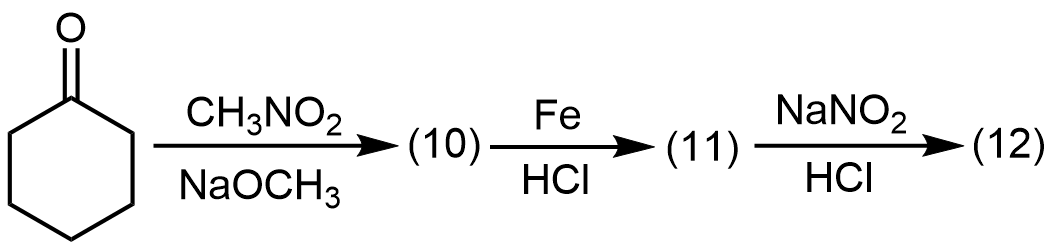
\includegraphics[scale=0.38, valign=c]{./Figure/2011/2011_1_4.png}
    \item 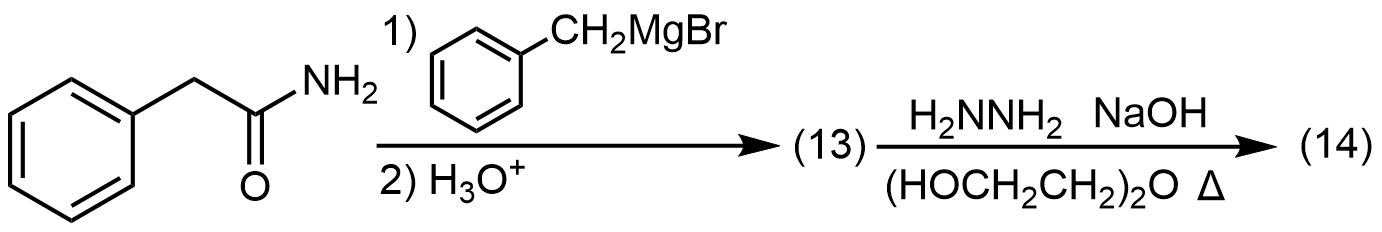
\includegraphics[scale=0.38, valign=c]{./Figure/2011/2011_1_5.png}
    \item 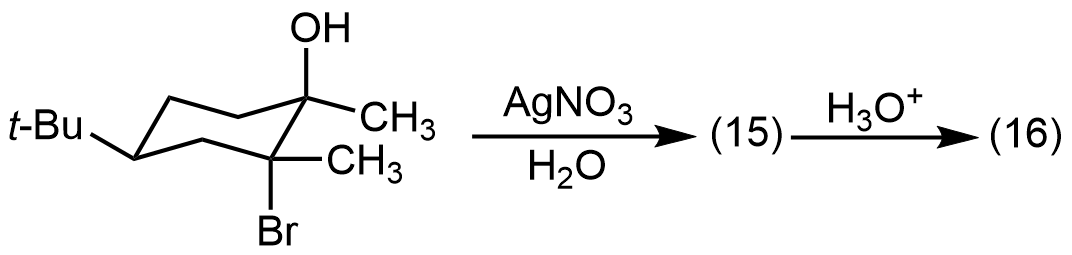
\includegraphics[scale=0.38, valign=c]{./Figure/2011/2011_1_6.png}
    \item 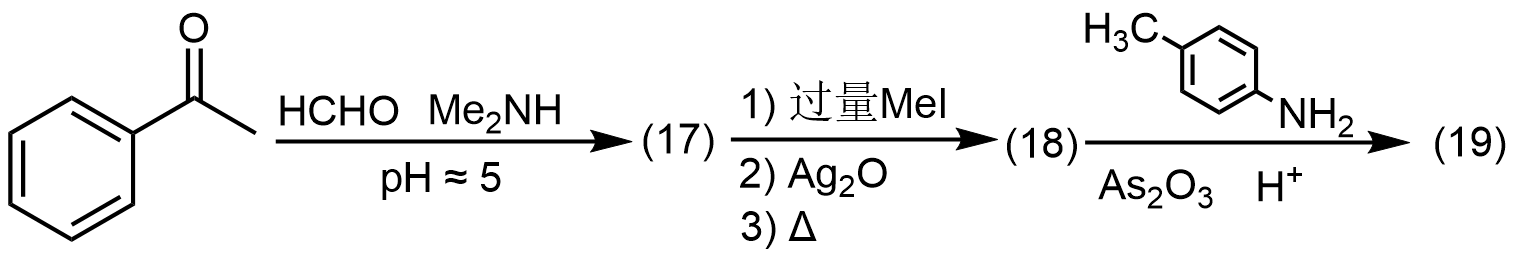
\includegraphics[scale=0.38, valign=c]{./Figure/2011/2011_1_7.png}
    \item 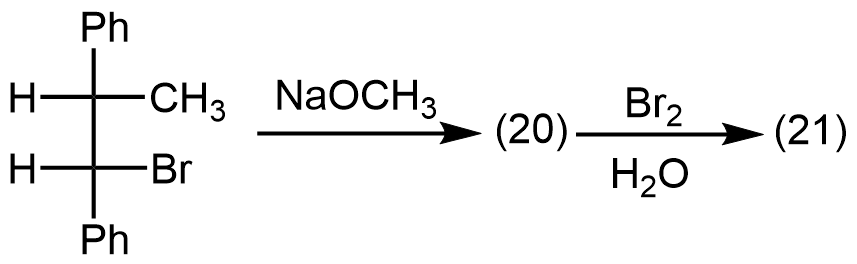
\includegraphics[scale=0.38, valign=c]{./Figure/2011/2011_1_8.png}
    \item 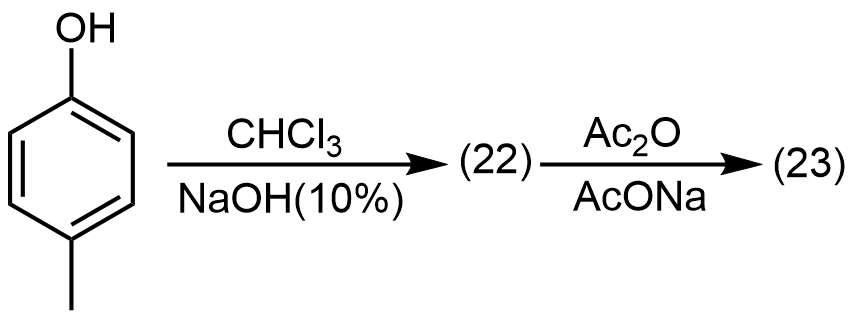
\includegraphics[scale=0.38, valign=c]{./Figure/2011/2011_1_9.png}
    \item 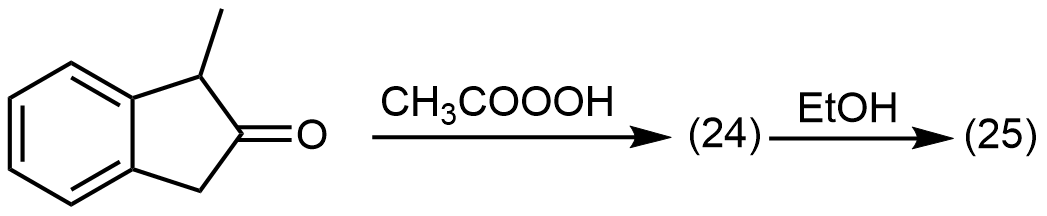
\includegraphics[scale=0.38, valign=c]{./Figure/2011/2011_1_10.png}

\end{enumerate}

\vspace{0.5cm}
\noindent\textbf{二、机理题(30 pts.)}

\begin{enumerate}[label=\arabic*., start=1, itemsep=1.5ex]
    \item 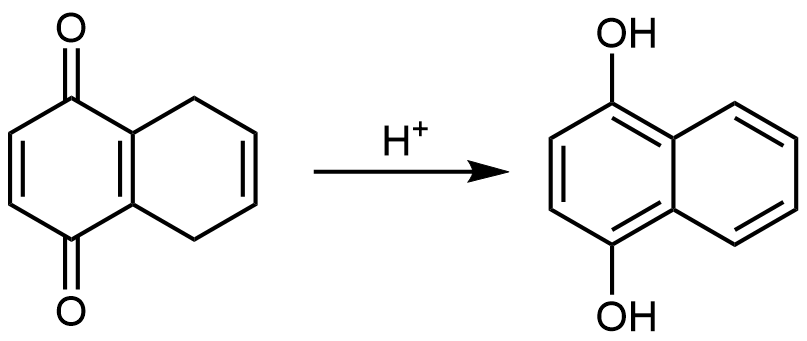
\includegraphics[scale=0.38, valign=c]{./Figure/2011/2011_2_1.png}
    \item 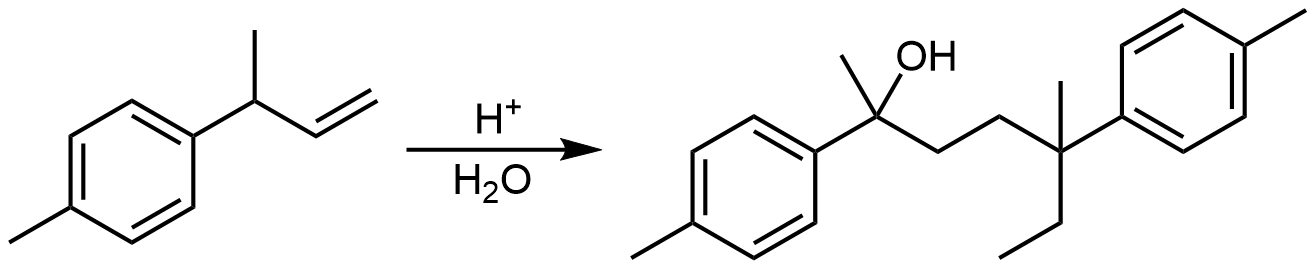
\includegraphics[scale=0.38, valign=c]{./Figure/2011/2011_2_2.png}
    \item 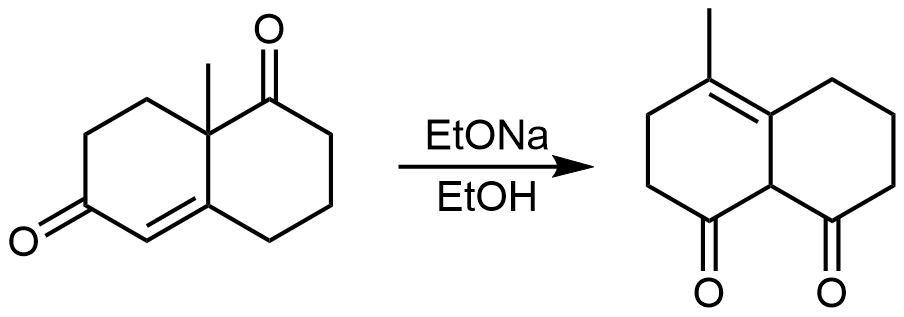
\includegraphics[scale=0.38, valign=c]{./Figure/2011/2011_2_3.png}
\end{enumerate}

\vspace{0.5cm}
\noindent\textbf{三、合成题(30 pts.)}

\begin{enumerate}[label=\arabic*., start=1, itemsep=1.5ex]

    \begin{figure}[htbp]
        \centering
        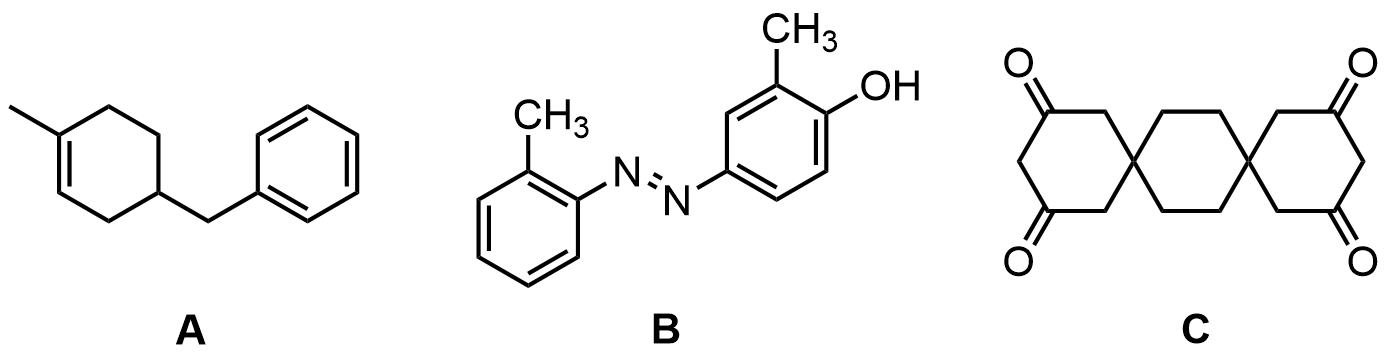
\includegraphics[scale=0.38]{./Figure/2011/2011_3.png}
    \end{figure}
    \item 以苯及小于等于2个碳的有机物为原料及必要的无机试剂合成\textbf{A}
    \item 以苯及小于等于2个碳的有机物为原料及必要的无机试剂合成\textbf{B}
    \item 以小于等于2个碳的有机物为原料及必要的无机试剂合成1,4-环己二酮，再以1,4-环己二酮及小于等于3个碳的有机物为原料及必要的无机试剂合成\textbf{C}
\end{enumerate}

\newpage

\vspace{0.5cm}
\noindent\textbf{四、综合题(20 pts.)}

\begin{figure}[htbp]
    \centering
    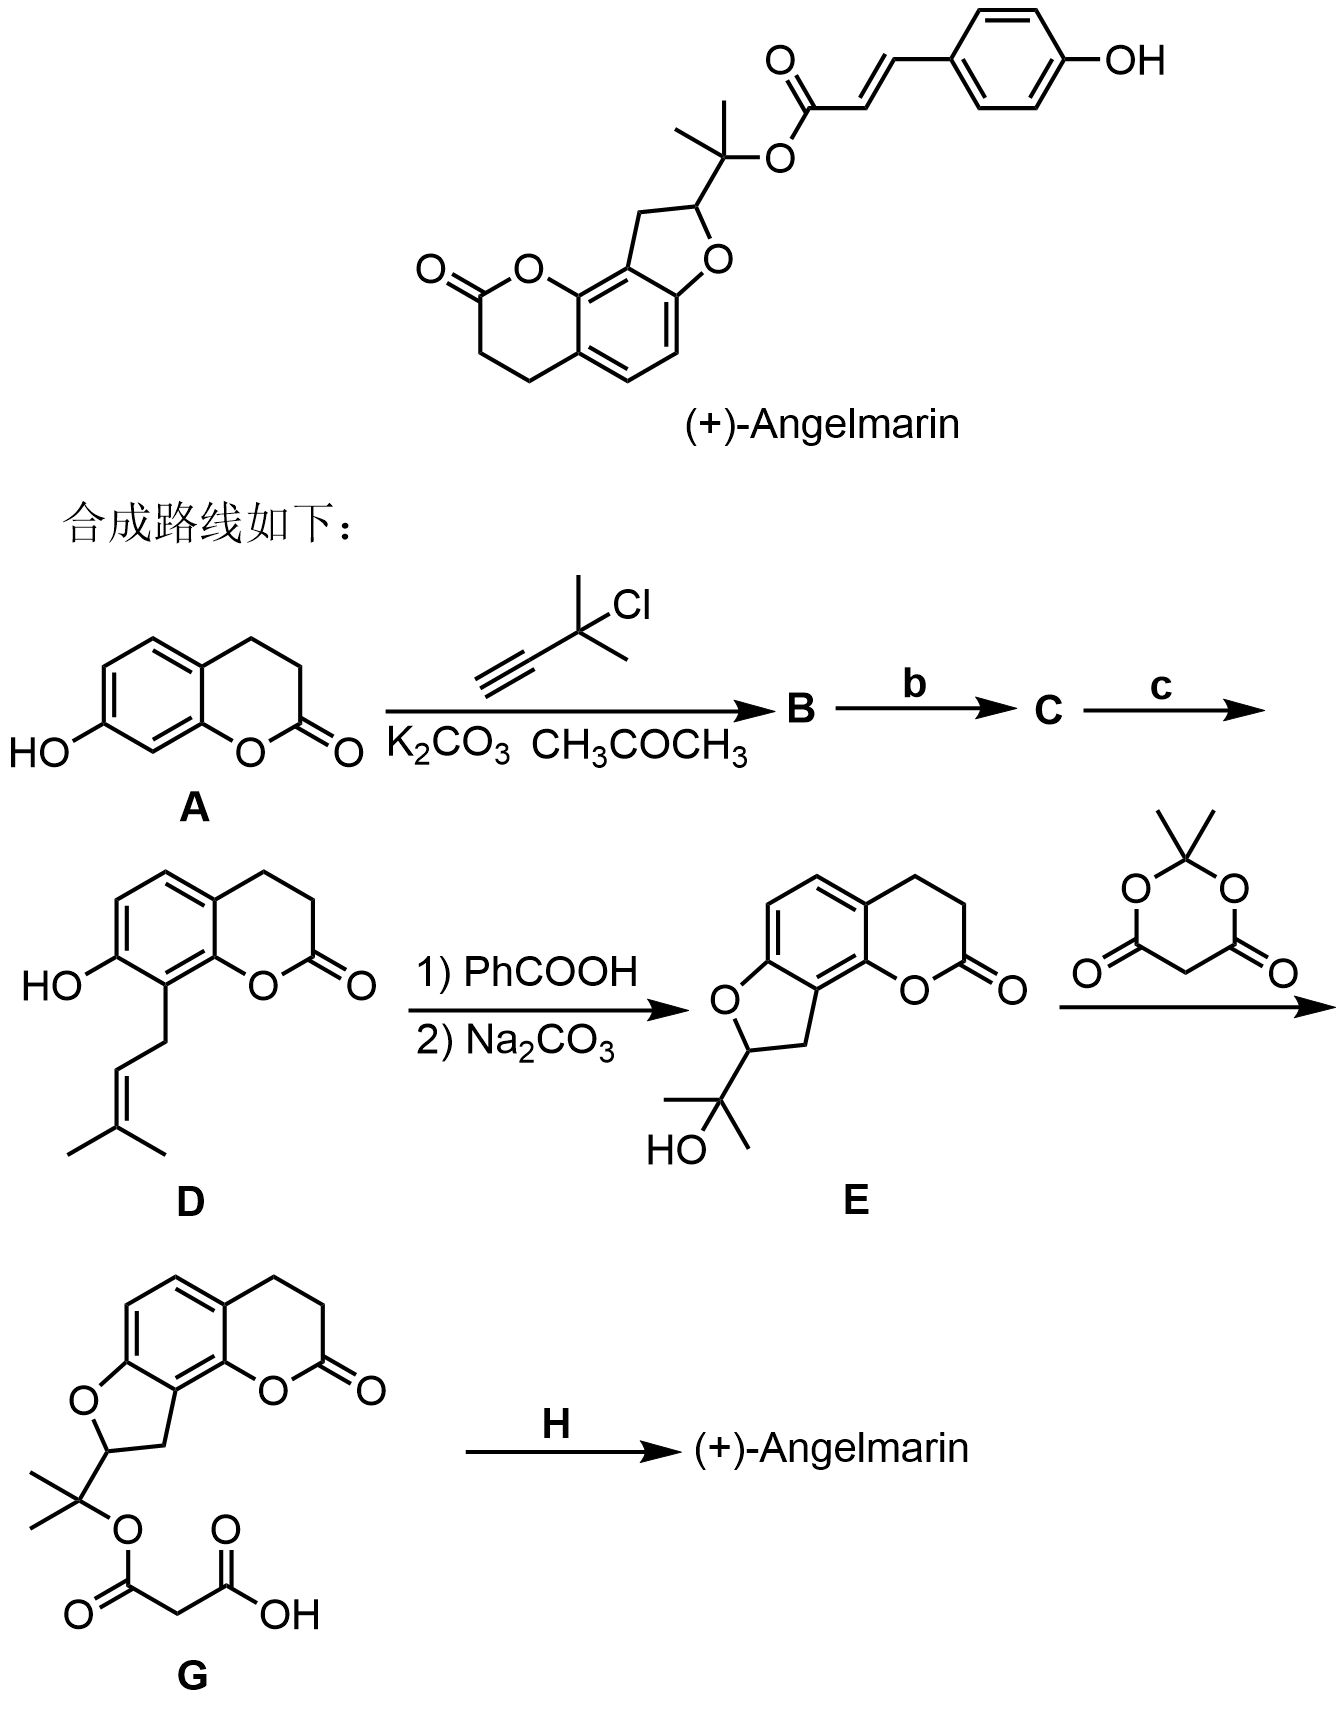
\includegraphics[scale=0.37]{./Figure/2011/2011_4.png}
\end{figure}

\begin{enumerate}[label=\arabic*., itemsep=1.2ex]
    \item 写出中间产物B，C和从G合成(+)-Angelmarin所需的化合物H的结构式。(3pts.)
    \item 写出从$\ce{B}$到$\ce{C}$的反应条件$\boldsymbol{1}$、以及从$\ce{C}$到$\ce{D}$的反应条件$\boldsymbol{2}$。(2 pts.)
    \item 化合物$\ce{A}$可以由乙酸酐通过Perkin反应得到，写出另外两种主要原料。(2 pts.)
    \item 3-甲基-3-氯-1-丁炔是合成中的原料之一，以乙炔和必要的有机、无机试剂，用不超过三步的反应合成该化合物。(5 pts.)
    \item 写出从$\ce{D}$到$\ce{E}$的反应历程。(8 pts.)
\end{enumerate}

\vspace{0.5cm}
\noindent\textbf{五、实验题 略}